% !TEX TS-program = pdflatex
% !TEX encoding = UTF-8 Unicode

% This is a simple template for a LaTeX document using the "article" class.
% See "book", "report", "letter" for other types of document.

\documentclass[12pt]{report} % use larger type; default would be 10pt

\usepackage[utf8]{inputenc} % set input encoding (not needed with XeLaTeX)

%%% Examples of Article customizations
% These packages are optional, depending whether you want the features they provide.
% See the LaTeX Companion or other references for full information.

%%% PAGE DIMENSIONS
\usepackage{geometry} % to change the page dimensions
\geometry{a4paper} % or letterpaper (US) or a5paper or....
% \geometry{margin=2in} % for example, change the margins to 2 inches all round
% \geometry{landscape} % set up the page for landscape
%   read geometry.pdf for detailed page layout information

\usepackage{graphicx} % support the \includegraphics command and options

% \usepackage[parfill]{parskip} % Activate to begin paragraphs with an empty line rather than an indent

%%% PACKAGES
\usepackage{booktabs} % for much better looking tables
\usepackage{array} % for better arrays (eg matrices) in maths
\usepackage{paralist} % very flexible & customisable lists (eg. enumerate/itemize, etc.)
\usepackage{verbatim} % adds environment for commenting out blocks of text & for better verbatim
\usepackage{subfig} % make it possible to include more than one captioned figure/table in a single float
\usepackage[final]{pdfpages}
% These packages are all incorporated in the memoir class to one degree or another...

%%% HEADERS & FOOTERS
\usepackage{fancyhdr} % This should be set AFTER setting up the page geometry
\pagestyle{fancy} % options: empty , plain , fancy
\renewcommand{\headrulewidth}{0pt} % customise the layout...
\lhead{}\chead{}\rhead{}
\lfoot{}\cfoot{\thepage}\rfoot{}

%%% SECTION TITLE APPEARANCE
\usepackage{sectsty}
\allsectionsfont{\sffamily\mdseries\upshape} % (See the fntguide.pdf for font help)
% (This matches ConTeXt defaults)

%%% RULE

\newcommand{\HRule}{\rule{\linewidth}{0.5mm}}

%%% BIBLIOGRAPHY

\usepackage{apacite}                           %bibliography in apa-style

%%% ToC (table of contents) APPEARANCE
\usepackage[nottoc,notlof,notlot]{tocbibind} % Put the bibliography in the ToC
\usepackage[titles,subfigure]{tocloft} % Alter the style of the Table of Contents
\renewcommand{\cftsecfont}{\rmfamily\mdseries\upshape}
\renewcommand{\cftsecpagefont}{\rmfamily\mdseries\upshape} % No bold!

\setcounter{secnumdepth}{-2}

%%% TABLES

\renewcommand{\arraystretch}{1.2}

%%% END Article customizations

%%% The "real" document content comes below...

\begin{document}

\begin{titlepage}

\begin{center}


% Upper part of the page

\includegraphics[width=1\textwidth]{./logo}\\[1cm]    

\textsc{\Large Bachelor Thesis}\\[0.5cm]
\textsc{\Large {[}201000166{]}}\\[0.5cm]


% Title
\HRule \\[0.4cm]
{ \huge \bfseries Research Proposal}\\[0.4cm]

\HRule \\[1.5cm]

% Author and supervisor
\begin{minipage}{0.4\textwidth}
\begin{flushleft} \large
\emph{Author:}\\
Micha \textsc{van den Enk} \\
{[}s1004654{]} \\
\end{flushleft}
\end{minipage}
\begin{minipage}{0.4\textwidth}
\begin{flushright} \large
\emph{Supervisors:} \\
Dr. H. H. \textsc{Leemkuil} \\
Second \textsc{supervisor} \\
\end{flushright}
\end{minipage}

\vfill

% Bottom of the page
{\large DATE}

\end{center}

\end{titlepage}

\tableofcontents

\chapter{Preface}

In this document the reader can find a proposal for designing a course on quantum mechanics in a qCraft learning environment. This is an assignment executed for a bachelor thesis. The document contains a table with general information, a short summary of the assignment, a detailed description of the assignment, the design approach and a planning. The general information section contains a table with data about the context of the assignment. The summary provides a short description of the product. The detailed description contains background information, information about the content of the instruction, a description of the technology used for the instruction and a conceptual framework. The design approach gives an outline of what will take place in order to develop the instruction: what analyses will take place, how the literature study will be conducted, how the information of the analyses and the literature study will be used in the design, how the instruction will be developed, how the instruction will be evaluated, and what the conclusion and discussion section will contain. Finallly, there is a planning included for the process of the bachelor thesis.

\chapter{General Information}

\begin{table}[h]
\begin{center}
\begin{tabular}{ l p{8cm} }
Researcher & Micha van den Enk (s1004654) \\
Study & Onderwijskunde \\
Study Department & Instructional Technology \\ 
Date & \\
First supervisor & Dr H. H. Leemkuil \\
Second supervisor & \\
Keywords & Quantum mechanics, Middle school Education, Netherlands \\
Title & \\
\end{tabular}
\end{center}
\caption{\footnotesize General information about the bachelor thesis}
\end{table}

\chapter{Summary}



\chapter{Description}

This chapter contains a short description of the background of the subject matter on middle schools in the Netherlands, the content of the instruction itself, the technology which will be used for the instruction, and an outline of the conceptual framework for the literature study.

\section{Background}

In the Netherlands, quantum mechanics always used to be a topic which schools themselves could choose to teach or not to teach. The only skill students had to know for the Centraal Eindexamen (the national central exams at the end of high school) which comes close to quantum mechanics is to elucidate the photoelectric and the wave-particle duality, mentioned within point 20 under subdomain E3 (citation eindexamenblad). However, one of the changes in the Centraal Eindexamen of 2016 was the addition of domain F1, which is called Quantum world. For this subdomain the candidate has to be able to apply the wave-particle duality and the uncertainty principle of Heisenberg, and to explain the quantization of energy levels in some examples with a simple quantum physical model. In order to give all candidates a chance of passing this subdomain, schools have to alter their programs in order to meet the expectations of the Centraal Eindexamen.

However, when searching the internet using the search machine Google concerning the implementation of quantum mechanics in Dutch high schools, the quantity and the quality of the results are very low. There are also no results to be found in the Dutch papers. An example is the Dutch site http://www.quantumuniverse.nl/, where teachers can find a small amount of brief courses on fundamental quantum mechanics, and where the forums are very quiet with only 5 discussions, of which 4 are just started threads from the site administrator.

Upon finding this information, an expert was consulted to confirm this conjecture. The expert was researching the implementation of quantum mechanics on middle schools, and she also a first degree physics teacher. She stated that within her school there were no initiatives to bring this topic in their classrooms, and that their school was no exception as well.

The fact that next year domain F1 has to be fully implemented and teached to all vwo students who chose physics as an examination subject is therefore slowly turning into a sword of Damocles. This stresses the urgency for the development of new course material.

\section{Content}

Quantum is not the most easy topic to introduce to physics. The subject is very counterintuitive, and still poses headaches to many physicists today. The great physicist Richard Feynman is known for saying: “I think I can safely say that nobody understands quantum mechanics” (1965), and this statement still holds. Quantum mechanics is this counterintuitive because it contradicts a lot of axioms we inherited from classical physics. These contradictions are highlighted by an article written by Einstein, Podolsky and Rosen, which states that the current understanding of quantum mechanics contradict the criterion of reality and the hypothesis of locality.

There are a lot of resources available for teaching quantum mechanics. Most of these resources are academical and focus on teaching the mathematics. Their philosophy is that the student can only really get a grasp on quantum mechanics if he understand the underlying mathematical mechanics. An example of such a resource is \citeA{qumech}. These resources are not very usefull when teaching middle school students, because it demands an understanding of mathematics which is beyond the knowledge of middle school students, for example the integration of Schröder equations.

The other way of teaching quantum mechanics is by teaching the key principles of quantum mechanics. A fashion in which this could be achieved is by only considering the perfectly correlating instances. An example of such an instance is quantum teleportation. \citeA{dance} explains this phenomenon without having to resort to very complex mathematics, but still explaining the fundamentals of quantum mechanics, namely observer dependency, superposition and quantum entanglement. The instruction will therefore use quantum teleportation to explain these three fundamental principles, so the learner will gain a concepual understanding of quantum mechanics.

\section{Technology}

The course will make use of qCraft, a modification made by members of Google for the game Minecraft. This game supports an accessible way for the player to get introduced and to interact with the aforementioned principles superposition, observer dependency and entanglement.

First, a short introduction is given which broadly describes the current state of research in Game-Based Learning. Then the concept of the game Minecraft is outlined, first by specifying the game mechanics and secondly by portraying the potentials for the game being a fit learning environment. This is followed by a depiction of the modification qCraft itself, consisting of a description of what qCraft adds to Minecraft and how this can be beneficial for learning quantum mechanics. 

\subsection{Minecraft}

\subsubsection{Mechanics}

Minecraft is a sandbox game developed by Mojang which can at best be described as a first-person Lego game: the player controls an Avatar who moves around in a three-dimensional world which consists of blocks, all being 1 cubic meter in size. The terrain generator uses a seed to randomly create a terrain. The player can move through walking, running and jumping around in the world. The blocks are the atoms of the game: they are the smallest components of the game and they can be instances of certain block-types, which can be compared to atoms as instances of different elements. Every element has its own texture and mechanics. Some block-types can be found naturally in the world, other block-types can only be crafted by combining other items together in a crafting recipe. Next to the blocks, the player can also find entities in the game called mobs, which can be friendly animals or destructive monsters. Animals are generated with the terrain generator, but they also have a rare chance of spawning randomly. Monsters only spawn randomly if the right spawning conditions are met. In the settings these mobs can be turned on or off. Finally, the game also contains items. Most of the time these are just portable versions of the aforementioned blocks, but there are also items which cannot be placed as blocks. The latter are most of the time utility items like maps, clocks or tools. The player also has an inventory in which he can store items for later use. A full list of blocks, entities, items and mechanics can be found on the minecraft wiki: http://minecraft.gamepedia.com/.

As in version 1.7 of minecraft, there are three different game modes: Survival Mode, Creative Mode and Adventure Mode. In Survival Mode, the player can find and harvest blocks in order to gain items, which can be placed somewhere else in the world as blocks or use them in crafting recipes to create different blocks. In order to harvest the blocks, the player sometimes has to use different tools, e.g. he has to use a pickaxe to mine stone blocks. Other blocks can be harvested with the players bare hands, but can often still be harvested faster when using a tool, e.g. dirt can be harvested faster with a shovel. The player also has a health bar, a hunger bar and an experience bar. If his health drops to zero, he drops all the items in his inventory on the spot and dies. He will then respawn at his original spawning point or next to the bed he most recently slept in. If his hunger bar drops to zero, the player slowly loses health. The player has to eat in order to raise his food bar, and if his  food bar is completely full, the player also will regenerate health. Finally, the player can gain experience points from certain tasks. This can be harvesting certain blocks or slaying mobs. By getting experience, the player can obtain levels. These levels can be spend on enchanting, which enhances certain weapons or tools. The focus of Survival Mode is therefore on staying alive, harvesting blocks, setting up farms in order to get certain items like food, getting tools, weapons and armors, and building a nice home.

In Creative Mode, the player already has all of the blocks in his disposal. The player also has the power of flight. The focus of Creative Mode is more on building than survival mode, because the player is less restricted and can therefore build whatever he wants to build within  the general restrictions of the game.

The mode which was added most recently to minecraft in version 1.7 is Adventure Mode. This mode is very similar to survival mode, except that the player is not able to destroy blocks. This mode is often used in so called adventure maps, which are premade maps which the player can explore or complete.

Minecraft can be played singleplayer or multiplayer. If played multiplayer, someone sets up a server, which the players connect to with their own minecraft client. They then control their own avatar and can interact with each other by chat or by altering the world.
Minecraft as a learning environment

Minecraft has great potential as a learning environment. Foremost, a lot of people think of Minecraft as fun to play, so students are motivated to learn in Minecraft and are engaged in completing the learning tasks. This is partly because the player can do a lot of different things in the game and therefore enhancing the gameplay for himself. Another reason is that Minecraft is a game that is highly creative, which is also appealing towards a lot of players. Sequently, players learn from the game by interacting with the world and observing the result. This is called Discovery Learning, which is a powerful learning method. For example, a player can learn about different architectural styles by trying to build a house for him to live in or by building gigantic buildings in Creative Mode. Another example is learning how to use redstone. Redstone is used to build logical circuits, quite like programming in Assembly. There are players who construct highly complex contraptions with redstone, like computers or robots. Minecraft also has the advantage of different players collaborating in one world. This way they can enhance each other's learning by discussing and showing each other contraptions or buildings without having to share one single screen. Minecraft is currently also the best sold PC game and therefore has a large active community, in which members upload tutorials on building certain contraptions on YouTube, maintain a wiki to share knowledge with each other and build different modifications for the game in order to extend the gameplay, like qCraft.

Minecraft is already being used in order to facilitate learning on schools, made possible by an elementary school teacher who launched the MinecraftEdu project. He teaches with Minecraft by giving his students tasks within the game, like building a house with  certain restrictions. This can be viewed on his YouTube channel https://www.youtube.com/user/MinecraftTeachr. Giving tasks enables the students to be very creative in completing the task. A more guided version of using Minecraft for education is by building certain premade map. By doing this, the student doesn't have an infinite world he can explore anymore because he is restricted by the boundaries of the map. The player is also only able to use the resources which are given to him in the map. This way the teacher can organize the learning task for the students so they can focus on the learning tasks instead on exploring aspects of the game which are irrelevant  for the learning tasks, which leads to saving time and cognitive load. The teacher can guide the learning task even more by presenting texts. The teacher can drop books in the map for the player to read, he can place signs with short messages and he can even display text in the chat. He can also reward the students for completing certain tasks by presenting special items, opening new parts of the map and giving experience points. This provides the students with motivation to engage in more tasks. If the teacher knows how to program in Java, he can even create his own modifications for Minecraft in order to teach something which cannot be teached with the vanilla game.

There are also some drawbacks of using Minecraft for teaching. One of them is that Minecraft is not a very realistic simulation, so the learning opportunities come mostly in the form of analogies. Another drawback is that both teacher and student have to learn how to play Minecraft before they can construct premade maps or learn from playing the game.
qCraft

\subsubsection{qCraft}

qCraft is a modification for Minecraft which adds four principles of quantum mechanics to minecraft. It is developed in order to teach quantum mechanics to players in an intuitive game. Because of this, qCraft can be qualified as an educational game. The introduced principles of quantum mechanics are Observational Dependency, Superposition, Entanglement and Quantum Teleportation. Observational dependency is implemented by introducing observational dependent blocks, which behave like different block-types depending on the angle from which the player views the block. Superpositional blocks are similar to observational dependent blocks, with the difference that only the dimension in which the player is standing matters and that the block metamorphoses to different block-types at random if the player observes the block. Blocks can also be entangled, this means that if one of the blocks takes on a block-type, all entangled blocks also take that same block-type. Quantum Teleportation is implemented in two ways, one way swaps blocks of a certain area with the blocks of a certain other area, the other way teleports the player itself from one portal to a connected other portal.

\subsubsection{Learning opportunities of qCraft}

In the very least, the player can learn about quantum mechanics by tangential learning. This is the concept of confronting players with a certain name or concepts, him getting curious and researching the name or concept and thereby learning more about it. A famous example is the adversary from the game Final Fantasy VII which is called Sephiroth. Although it was just a name without it having any influence on the game, players still got curious where the name came from and thereby learned about the Sephirot in Jewish Kabbalah. The same way a player of qCraft could encounter the word "Entanglement", getting curious and looking up on the internet what it is. A problem with tangential learning is that not everybody will be curious enough in order to research certain names or that some players will not notice the name to be special.

However, qCraft does more than only tangential learning. As already mentioned before, Minecraft is a mighty tool for discovery learning. By discovering the properties of the blocks introduced by qCraft and using these blocks for building or puzzle solving, the player can develop an intuition for these principles, which can lead to better understanding quantum mechanics. Even better, he can do so in a way that is fun and engaging. However, this intuition does not necessarily lead to better understanding of quantum mechanics, because the principles of qCraft are not directly linked to real quantum mechanics. However, when using a premade map, the map designer can put texts in the map in which the properties of the qCraft block-types can be directly linked to how it works in reality. Finally, the mod could raise awareness about the implications and the potential of quantum mechanics and thereby it could persuade the player to think of quantum mechanics as important.

\section{Conceptual framework}

The use of games for educational purposes is called GBL. Relatively speaking, only little research has been carried out to investigate GBL, but recent reviews revealed a potential of games being an effective tool for instruction, "even more effective than conventional instruction" \cite[p.~1]{wouters}. In order for GBL to take place, the game has to supersede sole entertainment purposes by having an educational value, so that the player learns something about the real world by playing the game. Examples of these games are historical games like Assassin's Creed, Age of Empires or Valiant Hearts, in which the player is exposed to certain historical events or figures, or puzzle games like Portal, in which the player develops an understanding about physics. However. these games are often only intended for entertainment purposes and are only tangentially fit for educational purposes. Most research within GBL is conducted on games which are specifically designed to have an educational value. These games often contain explicit formulated learning goals which can be tested by pre- and post-testing. They are designed with the primary goal of education rather than entertainment, and are therefore a subset of Serious Games. This term refers to the set of games designed for a primary goal other than pure entertainment. This goal can be teaching, but also raising awareness about a certain topic or persuading the player to believe something.

\citeA{smithragan} list different kinds of learning, and of these kinds this instruction will be focused on \emph{concept learning} and \emph{principle learning}. The instruction will be structured according to the events of instruction \cite{smithragan} (see table~\ref{tab:eventsinstruction}). These events can be filled in in a supplantive manner or in a generative manner. When the event is supplantive, the instruction will already supply the education in such a way that the learner does not have to elaborate for himself, for example by using scaffolding. A generative event however will let the learner elaborate the education for himself, for example by asking questions about the material. It is important to note that most events are not entirely supplantive or generative but are somewhere in between.

The game will be used to let the student discover the principles for himself by using the learning environment. This strategy of teaching is called \emph{inquiry strategy} \cite{smithragan}, fitting within constructivist theories. When using the inquiry strategy, the events should be more generative than supplantive.

\begin{table}
\begin{tabular}{| p{7cm} | p{7cm} |}
\hline
\multicolumn{2}{|c|}{\scshape Expanded Events of Instruction}\\ \hline
Generative & Supplantive \\ \hline
\multicolumn{2}{|c|}{\textbf{Introduction}} \\ \hline
Activate attention to activity & Gain attention to learning activity \\ \hline
Establish purpose & Inform learner of purpose \\ \hline
Arouse interest and motivation & Stimulate recall of prior knowledge \\ \hline
Preview learning activity & Provide overview \\ \hline
\multicolumn{2}{|c|}{\textbf{Body}} \\ \hline
Recall relevant prior knowledge & Stimulate recall of prior knowledge \\ \hline
Process information and examples & Present information and examples \\ \hline
Focus attention & Gain and direct attention \\ \hline
Employ learning strategies & Guide or prompt use of learning strategies \\ \hline
Practice & Provide for and guide practice \\ \hline
Evaluate feedback & Provide feedback \\ \hline
\multicolumn{2}{|c|}{\textbf{Conclusion}} \\ \hline
Summarize and review & Provide summary and review \\ \hline
Transfer learning & Enhance transfer \\ \hline
Remotivate and cease & Provide remotivation and closure \\ \hline
\multicolumn{2}{|c|}{\textbf{Assessment}} \\ \hline
Assess learning & Conduct assessment \\ \hline
Evaluate feedback & Provide feedback and remediation \\ \hline
\end{tabular}
\caption{\footnotesize The Expanded Events of Instruction \protect \cite{smithragan} \label{tab:eventsinstruction}}
\end{table}

Another theory which will be used is the taxonomy of \citeA{bloom}. According to this taxonomy, learning objectives can be catched in six catagories:

\begin{enumerate}
\item Knowledge
\item Understanding
\item Application
\item Analysis
\item Synthesis
\item Evaluation
\end{enumerate}

These catagories all have their own appropriate action verbs, which will be used to formulate the learning goals for this instruction.

\chapter{Design approach}

A model which describes the process of developing educational resources is the Generic Model \cite{genericmodel} (see figure~\ref{fig:genmod}). It describes the phases Analysis, Design, Development, Implementation and Evaluation. This model will be partly used for this project. Because of time constraints and the limited size of the project it will only go as far as the horizontal bar of development, this will be elaborated further later in this chapter.

\begin{figure}[h]
\centering
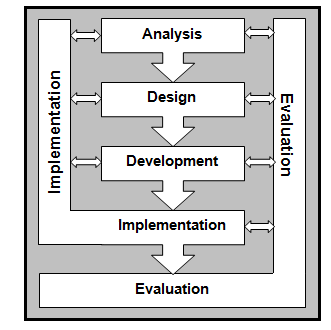
\includegraphics[width=0.7\textwidth]{genericmodel}
\caption{\footnotesize The generic model by \protect\citeA{genericmodel}\label{fig:genmod}}
\end{figure}

\section{Analyses}

The first step in the Generic Model \cite{genericmodel} is the step Analysis. In this step, data is gathered which is necessary for designing an effective solution. \citeA{smithragan} mention three different kinds of analysis, namely analyzing the learning context, analyzing the learners and analyzing the learning task.

\subsection{Analyzing the learning context}

A learning task always takes place in a certain learning context. In this case this is the middle school. It entails not only the place, but also the temporal and social environment \cite{smithragan}. The analysis of the learning context can provide the instructional needs and a description of the different factors influencing the instruction. With the instructional needs, the designer can establish the main learning goals for the instruction. The description of the learning environment can provide the learning opportunities and constraints which have to be taken into account for the instruction.

\subsection{Analyzing the learners}

The second analysis is that of the learners \cite{smithragan}. The purpose of this analysis is the characterization of the end user of the instruction, which is in this case the middle school students. For this analysis it is important to determine the similarities and differences between the learners. \citeA{smithragan} provide a list of factors which play a role in designing the instruction.

\subsection{Analyzing the learning task}

The final step is analyzing the learning task \cite{smithragan}. In this analysis the goals from the needs assessment during the analysis of the learning context have to be translated to test specifications, with which the content of the instruction can be established. In order to achieve these test specifications, first the type of learning has to be established. Having this established, the information-processing analysis can be conducted. Every type of learning has its own kind of information-processing analysis. \citeA{dance} will be used to conduct this information-processing analysis. The next step is the prerequisite analysis. The outcome of this has to correspond to the outcome of the learner analysis. Finally, the learning objectives can be written, which form the test specifications. Every learning objective has to contain a description of the terminal behavior or actions that will demontsrate learning, a description of the conditions of demonstration of that action and a description of the standard or criterion \cite{smithragan}. Every learning objective will fall into a catagory of Bloom his taxanomy of learning objectives \cite{bloom}, and will use appropriate action verbs. Most learning objectives within will be knowledge objectives, because there is a lot of new knowledge which has to be provided and it forms the basis for all other objectives. There will be no or very vew synthesis and evaluation objectives, because these objectives would take too much time within the instruction to achieve to be feasible to use.

\section{Literature Study}

After the analyses have been conducted, the literature study will take place. \citeA{lerencomm} state the different steps which go into doing literature research and writing the theoretic framework. The first step of the literature study will be considering the search terms. For this, the results of the analyses will have to be taken into account, especially the characterizations of the learners and the learning task. The search terms will then be expanded by finding synonyms and similar relevant terms by using the Thesaurus. After the search terms are determined, it has to be established which databases will provide useful results. Then a cyclic process will take place in which the amount of results will be assessed with these databases and search terms and then if needed the results are limited or expanded by using more search terms and filters. The results will always be constrained to peer-reviewed articles. Other filters could than be the recency of the articles or the educational level of the test subjects. When there is an appropriate amount of results, they will be filtered manually. First, the articles which seem relevant by their title and keywords will be selected. This will be done in a very broad sense, so only the really irrelevant results will be filtered out. These selected articles will then be skimmed by their abstract, introduction and conclusion and will be filtered out when they actually are not relevant. The remaining articles will then be used for constructing the theoretic framework. It could be that new keywords can be found in these articles. In this case this keyword will be added to the search terms in order to find even more results.

From the resulting articles a literature matrix will be constructed \cite{lerencomm}. This matrix will contain research questions in the top row and the resulting articles in the left row. By using this technique, every question can be answered per resulting article. The columns can then be summarized in order to answer every question separately. These answers ultimately are the content of the theoretic framework.

\section{Design}

The second phase of the Generic Model \cite{genericmodel} is the design phase. In this phase the results from the analyses are used to form design principles, which can be used to develop the instruction. There will be design principles for:
\begin{itemize}
\item a pretest for information about the preknowledge and the experience with playing games of the participants;
\item the text of the instruction;
\item the learning environment within Minecraft;
\item the posttest for testing the resulting knowledge of the participants.
\end{itemize}
Furthermore, a global design plan will be made, which is a distribution of the learning objectives over the course of the instruction. The basic hierarchy of the instruction will consist of the different learning events by \citeA{smithragan}.

\section{Development}

After the design phase comes the development phase, in which all the resources are finally fully developed, based on the earlier made design. This will be the developing of the pre- and posttest, the writing of the text and the developing of the learning environment in Minecraft. The development of the resources will be based on the earlier developed design principles and the global design plan.

\section{Formative Evalutation}

After the first development phase, the formative evaluations will take place. These evaluations are derived from the \emph{Evaluation Matchboard} \cite{evamatchboard}. After each evaluation, adjustments of the products have to take place as well. First, the resources will be screened to check whether the resources confirm to the design principles. Then, a focus group evaluation will take place. In this evaluation a subject matter expert will be interviewed to check whether the text contains statements which have to be adjusted or corrected with the current knowledge on quantum teleportation. Finally, a micro-evaluation will take place, in which the final product will be tested upon members of the target audience, or people similar to the target group audience. With this evaluation, the actual practicality can be tested by interviewing the participants. The actual effectiveness will also be tested by letting the participants make the posttest. The posttest will be open book, and ask mostly about learning objectives within \emph{understanding}, \emph{application} and \emph{analysis}.

\section{Implementation and Summative Evaluation}

The implementation and summative evaluation will not take place during this project. Implementation would be outside of the scope of the project, and could only be executed in a follow-up project. When proven to be succesful, the resources developed will be offered to MinecraftEdu, an organisation which has the mission to bring Minecraft into schools.

Because the lack of implementation, a summative evaluation is also out of the question. In order to conduct a succesful summative evaluation, the resources would have to be fully in use in the actual context, which is not the case for this project.

\section{Conclusion and Discussion}

When the micro-evaluation has taken place, the resulting data has to be processed and analyzed. With these results, a conclusion will be written down to summarize the advantages and drawbacks of the instruction. There also will be suggestions for improvement and for implementation.

\chapter{Planning}

All the steps in the design approach are to be ready in the week numbers mentioned in table~\ref{tab:planning}.

\begin{table}[h]
\begin{center}
\begin{tabular}{ l r }
Analyses & Week 18 \\
Literature research & Week 20 \\
Design & Week 21 \\
Development & Week 22 \\
Formative Evaluation & Week 24 \\
Conclusion/Discussion & Week 25 \\
Presentation & Week 26 \\
\end{tabular}
\end{center}
\caption{A general planning for the bachelor thesis \label{tab:planning}}
\end{table}

\bibliographystyle{apacite}
\bibliography{references}

\part{Appendix A: Evaluation matchboard}

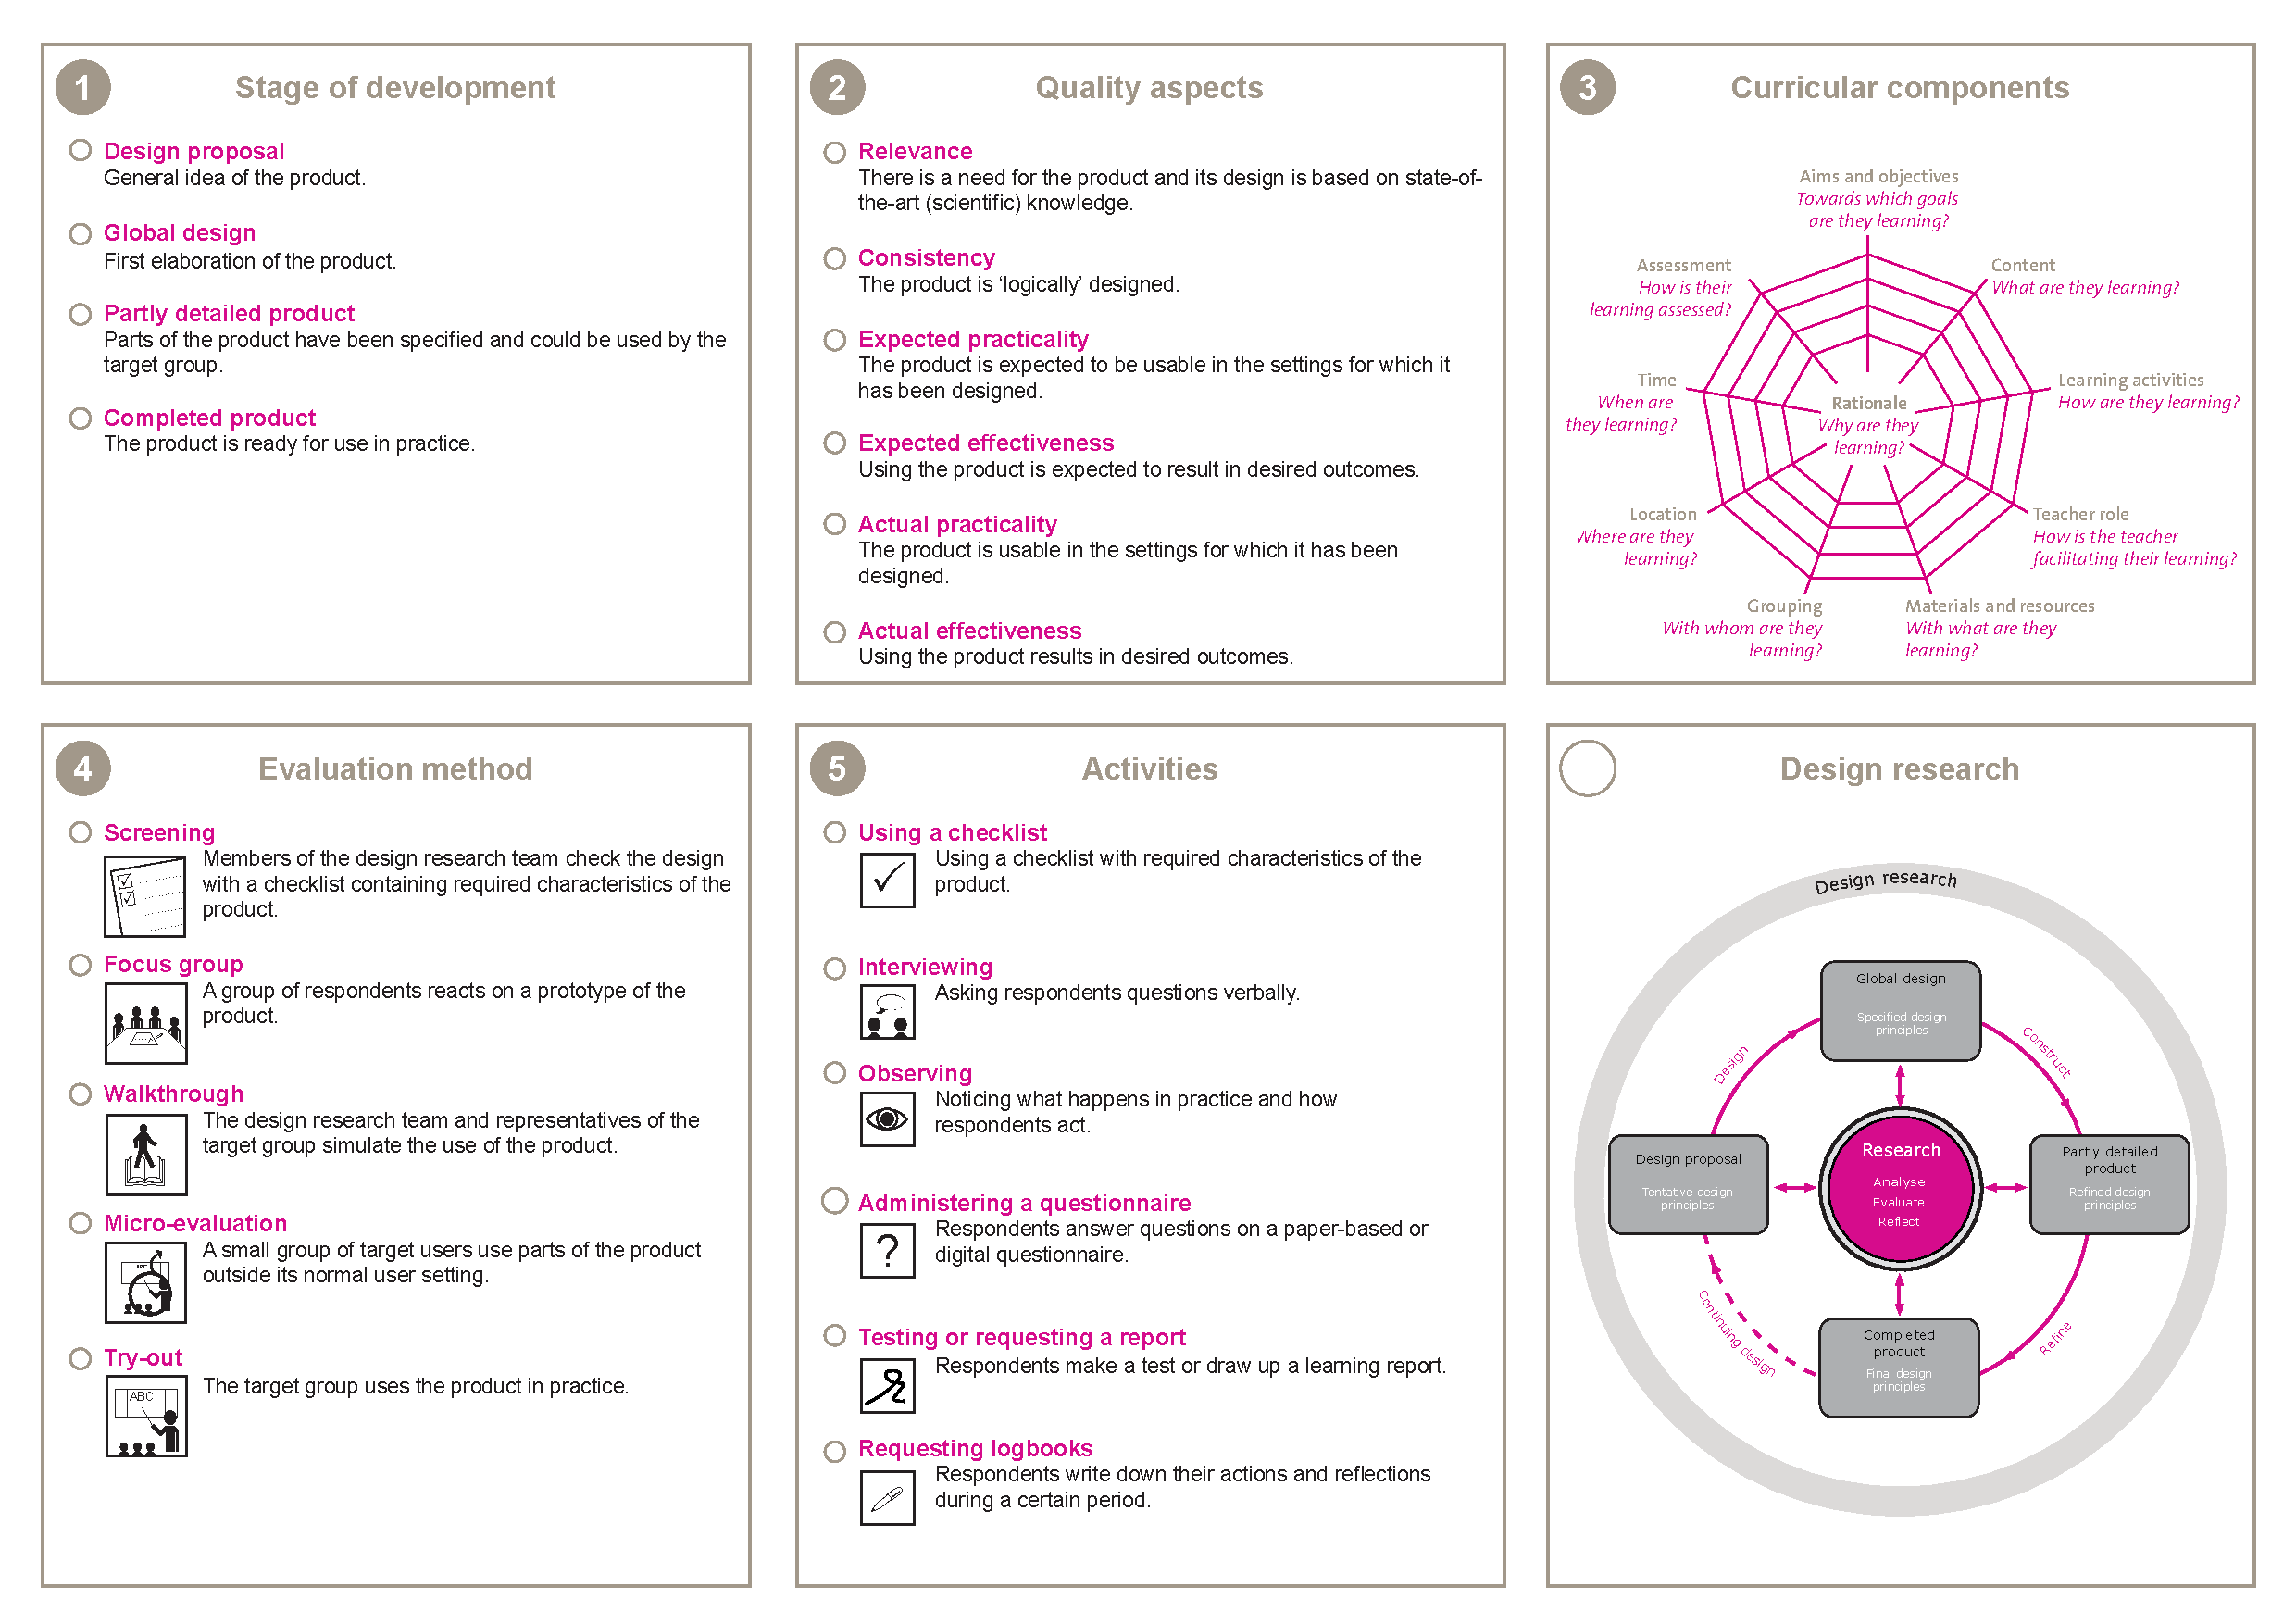
\includepdf[pages=-]{Evaluation_matchboard.pdf}

\end{document}
